% Provenance (never printed): see sources/outline_sources.md (Year 2: fractional
% crystallisation, Bowen's series, compatible and incompatible elements, mixing and
% assimilation, layered intrusions).
% Curves from figdata/bachelor-2/differentiation.py (Bowen 1913 plagioclase loop, Rayleigh and
% equilibrium laws, Wilcox 1954 Paricutin analyses and mass balance, AFC closed form,
% Tegner et al. 2023 Skaergaard whole-rock data); exercise and problem values in the Book 4
% scratch calculator calc/ch08.py.
\chapter{मैग्मीय विभेदन}\label{ch:b2:magmatic-differentiation}

20 फ़रवरी 1943 को मेक्सिको के पश्चिम में एक ज्वालामुखी फूटने लगा, और वह
नौ वर्ष तक फूटता रहा। उसके पहले लावा \qty{55}{\percent} सिलिका वाले बेसाल्टी
एंडेसाइट थे; उसके अंतिम लावा, फ़रवरी 1952 में,
\qty{60}{\percent} से थोड़ी अधिक सिलिका वाले एंडेसाइट थे। यह ज्वालामुखी, पारीकुटिन, इस बीच
किसी दूसरे स्रोत पर नहीं गया, और उसके लावा जैसे-जैसे निकले, एक के बाद एक विश्लेषित किए गए।
उसके नीचे का \omterm{def:b2:magma-emplacement:magma}{मैग्मा} स्वयं बदला: उसमें क्रिस्टल उगे और वह उन्हें पीछे छोड़ता गया, और उसने
अपने चारों ओर की कुछ ग्रेनाइटी चट्टान को खा लिया। जो \omterm{def:b2:magma-emplacement:magma}{मैग्मा} प्रावार से बेसाल्ट के रूप में निकलता है,
वह रायोलाइट के रूप में समाप्त हो सकता है, और रास्ते में वह जो चट्टानें पीछे छोड़ता है वे बताती हैं कि ऐसा कैसे हुआ।
यह अध्याय ठंडे होते \omterm{def:b2:magma-emplacement:magma}{मैग्मा} का अनुसरण करता है: खनिज किस क्रम में क्रिस्टलित होते हैं,
वे नियम जो बताते हैं कि क्रिस्टल हटाए जाने पर मुख्य और \omterm{def:b2:elements-in-the-earth:trace}{अनुरेखी तत्त्व} कैसे बदलते हैं,
उन क्रिस्टलों से बनी चट्टानें, और तब क्या होता है जब \omterm{def:b2:magma-emplacement:magma}{मैग्मा}
कोई दूसरा \omterm{def:b2:magma-emplacement:magma}{मैग्मा} या भूपर्पटी अपने भीतर ले लेता है।
% ledger: wilcox54:paricutin

\begin{recall}
\textbf{पुस्तक 2 (उच्च माध्यमिक) से}: आग्नेय चट्टानें और उनकी बनावटें; वह क्रम
जिसमें खनिज किसी बेसाल्टी \omterm{def:b2:magma-emplacement:magma}{मैग्मा} से क्रिस्टलित होते हैं, पहले ओलिवीन और अंत में क्वार्ट्ज़,
जो बोवेन के प्रयोगों से मिला। \textbf{रसायन-विज्ञान की पुस्तकों (द्वितीय वर्ष) से}:
द्विघटकी प्रावस्था आरेख, ठोस विलयन और उत्तोलक नियम।
\textbf{पुस्तक 3 (स्नातक वर्ष 1) से}: प्लैजियोक्लेज़, एनॉर्थाइट \ce{CaAl2Si2O8} और
एल्बाइट \ce{NaAlSi3O8} के बीच एक ठोस विलयन, और अन्य चट्टान-निर्माता सिलिकेट; आड़े
ध्रुवकों के बीच पतली काटें। \textbf{\cref{ch:b2:elements-in-the-earth} से}: खनिज--गलित और समग्र
विभाजन गुणांक, $\bar D = \sum_i x_i D_i$, संगत और \omterm{def:b2:elements-in-the-earth:partition}{असंगत
तत्त्व}, \omterm{def:b2:elements-in-the-earth:normalised}{प्रसामान्यीकृत आरेख} और \omterm{prop:b2:elements-in-the-earth:normalised}{यूरोपियम विसंगति}। \textbf{\cref{ch:b2:isotope-geochemistry} से}:
अनुरेखकों के रूप में समस्थानिक अनुपात और \omterm{prop:b2:isotope-geochemistry:mixing}{मिश्रण
अतिपरवलय}। \textbf{\cref{ch:b2:mantle-melting} से}: डायोप्साइड--एनॉर्थाइट
गलनक्रांतिक, \omterm{def:b2:mantle-melting:peritectic}{असर्वांगसम गलन}, त्रिघटकी आरेख और \omterm{def:b2:mantle-melting:primary}{प्राथमिक मैग्मा}।
\end{recall}

\section{क्रिस्टलन के अनुक्रम}\label{sec:b2:magmatic-differentiation:sequences}

बेसाल्टी \omterm{def:b2:magma-emplacement:magma}{मैग्मा} अपने सारे खनिज एक साथ क्रिस्टलित नहीं करता। बोवेन ने
प्रयोग से पाया कि ओलिवीन सामान्यतः सबसे पहले क्रिस्टलित होता है, 1200 और
\qty{1300}{\celsius} के बीच; कि कैल्शियम-समृद्ध प्लैजियोक्लेज़ लगभग वहीं शुरू होता है जहाँ पाइरॉक्सीन
शुरू होता है; और कि अंतिम, सिलिका-समृद्ध द्रव पोटैशियम फ़ेल्डस्पार, क्वार्ट्ज़ और
शायद मस्कोवाइट देता है, लगभग 750 से \qty{800}{\celsius} पर। इन दोनों के बीच मैफ़िक
खनिज केवल ढेर नहीं होते जाते: हर एक द्रव से अभिक्रिया करके अगला खनिज देता है।
% ledger: earle:bowen (Book 2), tulane:bowen (Book 2)

\begin{definition}[बोवेन की अभिक्रिया-श्रेणी]\label{def:b2:magmatic-differentiation:bowen}
\emph{बोवेन की अभिक्रिया-श्रेणी}\index{बोवेन की अभिक्रिया-श्रेणी} वह क्रम है जिसमें
सामान्य सिलिकेट ठंडे होते बेसाल्टी \omterm{def:b2:magma-emplacement:magma}{मैग्मा} से क्रिस्टलित होते हैं, दो शाखाओं के रूप में
जो अंत में मिलती हैं। \emph{असतत शाखा} में हर मैफ़िक खनिज
द्रव से अभिक्रिया करके किसी दूसरी संरचना का नया खनिज बनाता है: ओलिवीन,
पाइरॉक्सीन, एम्फ़ीबोल, बायोटाइट। \emph{सतत शाखा} में प्लैजियोक्लेज़
पूरे समय क्रिस्टलित होता रहता है, और उसका संघटन कैल्शियम-समृद्ध से सोडियम-समृद्ध
की ओर सतत बदलता है। अंतिम द्रव पोटैशियम फ़ेल्डस्पार, मस्कोवाइट और
क्वार्ट्ज़ क्रिस्टलित करता है।
\end{definition}
% ledger: earle:bowen (Book 2)

\begin{omfigure}
\centering
\begin{tikzpicture}[font=\small, x=1cm, y=1cm,
  mn/.style={draw, rounded corners=2pt, fill=white, inner sep=3pt, minimum width=2.3cm,
             align=center}]
\draw[-{Stealth[length=4pt]}, thick, gray] (-1.3,0.3) -- (-1.3,-6.0);
\node[rotate=90, anchor=south, font=\scriptsize, gray] at (-1.4,-2.85) {गिरता तापमान};
\node[anchor=east, font=\scriptsize] at (-1.5,0) {$\approx$ 1200--\qty{1300}{\celsius}};
\node[anchor=east, font=\scriptsize] at (-1.5,-5.6) {$\approx$ 750--\qty{800}{\celsius}};
\node[mn] (ol) at (1,0) {ओलिवीन};
\node[mn] (px) at (1,-1.4) {पाइरॉक्सीन};
\node[mn] (am) at (1,-2.8) {एम्फ़ीबोल};
\node[mn] (bt) at (1,-4.2) {बायोटाइट};
\draw[-{Stealth[length=4pt]}, thick] (ol) -- (px);
\draw[-{Stealth[length=4pt]}, thick] (px) -- (am);
\draw[-{Stealth[length=4pt]}, thick] (am) -- (bt);
\node[font=\scriptsize, align=center] at (1,0.8) {असतत शाखा\\(हर चरण पर एक नया खनिज)};
\node[mn] (ca) at (6,-1.4) {कैल्शियम-समृद्ध\\प्लैजियोक्लेज़};
\node[mn] (na) at (6,-4.2) {सोडियम-समृद्ध\\प्लैजियोक्लेज़};
\fill[left color=white, right color=white, top color=orange!35, bottom color=orange!8]
  (5.75,-2.0) rectangle (6.25,-3.6);
\draw[-{Stealth[length=4pt]}, thick] (ca) -- (na);
\node[font=\scriptsize, align=center] at (6,0.8) {सतत शाखा\\(एक खनिज, बदलता संघटन)};
\node[mn, minimum width=7.2cm] (last) at (3.5,-5.6) {पोटैशियम फ़ेल्डस्पार, मस्कोवाइट, क्वार्ट्ज़};
\draw[-{Stealth[length=4pt]}, thick] (bt) -- (bt|-last.north);
\draw[-{Stealth[length=4pt]}, thick] (na) -- (na|-last.north);
\end{tikzpicture}
\par\smallskip{\small \omterm{def:b2:magmatic-differentiation:bowen}{बोवेन की अभिक्रिया-श्रेणी}। ओलिवीन और कैल्शियम-समृद्ध प्लैजियोक्लेज़
बेसाल्टी \omterm{def:b2:magma-emplacement:magma}{मैग्मा} से सबसे पहले क्रिस्टलित होते हैं; बाईं ओर हर मैफ़िक खनिज द्रव से
अभिक्रिया करके अगला खनिज देता है, दाईं ओर प्लैजियोक्लेज़ सोडियम में निरंतर अधिक
समृद्ध होता जाता है; अंतिम, सिलिका-समृद्ध द्रव पोटैशियम फ़ेल्डस्पार, मस्कोवाइट और क्वार्ट्ज़ देता है।
तापमान निम्न दाब पर बेसाल्टी \omterm{def:b2:magma-emplacement:magma}{मैग्मा} के विशिष्ट मान हैं।}
\end{omfigure}
% ledger: earle:bowen (Book 2)

ये दो शाखाएँ \cref{ch:b2:mantle-melting} के दो प्रकार के प्रावस्था आरेखों के
संगत हैं। असतत अभिक्रिया एन्स्टेटाइट का उलटी दिशा में चलाया गया
\omterm{def:b2:mantle-melting:peritectic}{असर्वांगसम गलन} है: फ़ॉर्स्टेराइट के क्रिस्टल सिलिका में अधिक समृद्ध द्रव से अभिक्रिया करके
एन्स्टेटाइट देते हैं। सतत शाखा एक ठोस विलयन है। बोवेन ने इसे 1913 में
संश्लेषित प्लैजियोक्लेज़ों पर मापा, हर संघटन को एक ज्ञात तापमान पर रखकर और
काँच तथा क्रिस्टल खोजकर: एनॉर्थाइट \qty{1550}{\celsius} पर पिघलता है, एल्बाइट
लगभग \qty{1100}{\celsius} पर, और हर मध्यवर्ती प्लैजियोक्लेज़ एक अंतराल में पिघलता है,
एक निचले वक्र, सॉलिडस, और एक ऊपरी वक्र, लिक्विडस, के बीच (नीचे का
चित्र)।
% ledger: bowen13:plagioclase, bowen14:mgo-sio2

\begin{omfigure}
\centering
\begin{tikzpicture}
\begin{axis}[omrecord, width=0.78\linewidth, height=6.4cm,
  xmin=0, xmax=100, ymin=1050, ymax=1600,
  xlabel={एनॉर्थाइट (\unit{\percent}, आणविक)}, ylabel={तापमान (\unit{\celsius})},
  y tick label style={/pgf/number format/1000 sep={}}, unbounded coords=discard,
  tick label style={font=\scriptsize}, label style={font=\small}]
\addplot[very thick, black] table[x=an, y=T_liq] {figdata/out/bachelor-2-differentiation-plag-curve.dat};
\addplot[very thick, black, dashed] table[x=an, y=T_sol] {figdata/out/bachelor-2-differentiation-plag-curve.dat};
\addplot[only marks, mark=*, mark size=1.5pt, blue!70!black] table[x=an, y=T_liq] {figdata/out/bachelor-2-differentiation-plag-data.dat};
\addplot[only marks, mark=o, mark size=1.7pt, blue!70!black] table[x=an, y=T_sol] {figdata/out/bachelor-2-differentiation-plag-data.dat};
\draw[densely dotted, red!70!black, thick] (axis cs:50,1560) -- (axis cs:50,1287);
\draw[red!70!black, thick] (axis cs:50,1450) -- (axis cs:80.6,1450);
\draw[red!70!black, thick] (axis cs:33.3,1394) -- (axis cs:70.6,1394);
\draw[red!70!black, thick] (axis cs:13.9,1287) -- (axis cs:50,1287);
\addplot[only marks, mark=*, mark size=1.4pt, red!70!black] coordinates {(50,1450) (80.6,1450) (33.3,1394) (70.6,1394) (13.9,1287) (50,1287)};
\node[font=\scriptsize] at (axis cs:30,1530) {द्रव};
\node[font=\scriptsize, align=center] at (axis cs:83,1200) {प्लैजियोक्लेज़\\(ठोस विलयन)};
\node[font=\scriptsize, anchor=west] at (axis cs:2,1430) {लिक्विडस (ठोस रेखा)};
\node[font=\scriptsize, anchor=west] at (axis cs:42,1160) {सॉलिडस (डैश रेखा)};
\node[font=\scriptsize, anchor=south, red!70!black, fill=white, inner sep=1pt] at (axis cs:68,1452) {\qty{1450}{\celsius}};
\node[font=\scriptsize, anchor=north, red!70!black, fill=white, inner sep=1pt] at (axis cs:31,1284) {\qty{1287}{\celsius}};
\end{axis}
\end{tikzpicture}
\par\smallskip{\small वायुमंडलीय दाब पर प्लैजियोक्लेज़ फ़ेल्डस्पार, बोवेन (1913) के
शमन-प्रयोगों से: पिघलने का आरंभ (वृत्त) और समापन (बिंदु), मापों से होकर खींचे गए
वक्रों के साथ। लाल रंग में, \qty{50}{\percent} एनॉर्थाइट वाले द्रव का \omterm{def:b2:magmatic-differentiation:crystallisation}{साम्य क्रिस्टलन}:
\qty{1450}{\celsius} पर बने पहले क्रिस्टल में \qty{81}{\percent} एनॉर्थाइट है;
\qty{1394}{\celsius} पर \qty{71}{\percent} के क्रिस्टल \qty{33}{\percent} वाले द्रव के साथ
सहअस्तित्व में हैं; अंतिम द्रव में, \qty{1287}{\celsius} पर, \qty{14}{\percent} है
(\cref{exo:b2:magmatic-differentiation:1})।}
\end{omfigure}
% ledger: bowen13:plagioclase

ठोस विलयन क्रिस्टलित करने वाला द्रव उस घटक में समृद्ध होता जाता है जो
निम्नतर तापमान पर पिघलता है: \qty{50}{\percent} एनॉर्थाइट वाले द्रव से बने पहले प्लैजियोक्लेज़ में
\qty{81}{\percent} होता है, और द्रव
एल्बाइट की ओर बढ़ता है। आगे क्या होता है, यह इस पर निर्भर करता है कि क्रिस्टल
द्रव के संपर्क में बने रहते हैं या नहीं।

\begin{definition}[साम्य और भिन्नात्मक क्रिस्टलन]
\label{def:b2:magmatic-differentiation:crystallisation}
\emph{साम्य क्रिस्टलन}\index{साम्य क्रिस्टलन} में
क्रिस्टल अंत तक पूरे द्रव के साथ रासायनिक साम्य में रहते हैं, और द्रव के बदलने के साथ
फिर से साम्य में आते रहते हैं; तंत्र उसी संघटन के साथ समाप्त होता है
जिससे उसने आरंभ किया था। \emph{भिन्नात्मक क्रिस्टलन}\index{भिन्नात्मक क्रिस्टलन}
में हर क्रिस्टल, बनते ही, द्रव के साथ अभिक्रिया से अलग कर दिया जाता है:
नीचे बैठकर, कक्ष की दीवारों पर चिपककर, या बाद की वृद्धि से
ढक जाने पर; तब द्रव ऐसे विकसित होता है मानो क्रिस्टल
तंत्र से बाहर निकाल लिए गए हों।
\end{definition}

\omterm{def:b2:magmatic-differentiation:crystallisation}{साम्य क्रिस्टलन} में ऊपर के चित्र का प्लैजियोक्लेज़ बढ़ते हुए
\qty{81}{\percent} से \qty{50}{\percent} एनॉर्थाइट तक बदलता है, हर क्रिस्टल
द्रव के साथ विसरण द्वारा फिर से साम्य में आता रहता है, और अंतिम द्रव
सॉलिडस पर, \qty{1287}{\celsius} पर, लुप्त होता है। फ़ेल्डस्पार में विसरण धीमा है, और प्राकृतिक
क्रिस्टल शायद ही कभी साथ चल पाते हैं: हर क्रिस्टल का भीतरी भाग द्रव से कट जाता है,
जो तब \omterm{def:b2:magmatic-differentiation:crystallisation}{भिन्नात्मक क्रिस्टलन} की तरह व्यवहार करता है और एल्बाइट के निकट के संघटनों तक
जा सकता है। इस अध्याय के अंतिम खंड का एक चित्र दोनों पथों का परिकलन करता है।
% ledger: bowen13:plagioclase

\begin{definition}[द्रव का अवरोहण-पथ]\label{def:b2:magmatic-differentiation:lld}
किसी \omterm{def:b2:magma-emplacement:magma}{मैग्मा} का \emph{द्रव का अवरोहण-पथ}\index{द्रव का अवरोहण-पथ} उन संघटनों का
अनुक्रम है जो उसका द्रव क्रिस्टलित होते समय लेता है, किसी
विचरण आरेख या प्रावस्था आरेख पर आलेखित।
\end{definition}

\omterm{def:b2:magmatic-differentiation:lld}{द्रव का अवरोहण-पथ} केवल द्रव का गुण है। जो लावा अपने भीतर क्रिस्टल लिए हुए फूटे,
वे ठीक उस पर नहीं पड़ते, और विलकॉक्स ने, पारीकुटिन के लावाओं का अध्ययन करते हुए,
उनके पूर्ण-चट्टान विश्लेषणों और उनके आधारद्रव्य (द्रव भाग) के संघटनों, दोनों का उपयोग किया;
आधारद्रव्य का संघटन क्रिस्टलों को हटाकर परिकलित किया गया था।
% ledger: wilcox54:groundmass

\section{मुख्य तत्त्वों का भिन्नात्मक क्रिस्टलन}\label{sec:b2:magmatic-differentiation:majors}

क्रिस्टल हटाने से द्रव का संघटन सरल, रैखिक ढंग से बदलता है,
और इसे पढ़ने का सबसे पुराना साधन हर ऑक्साइड का सिलिका के विरुद्ध आलेख है।

\begin{definition}[हार्कर आरेख]\label{def:b2:magmatic-differentiation:harker}
\emph{हार्कर आरेख}\index{हार्कर आरेख} (सिलिका-विचरण आरेख) संबंधित चट्टानों के किसी समूह के
हर ऑक्साइड के द्रव्यमान-प्रतिशत को उनके \ce{SiO2} के द्रव्यमान-प्रतिशत के विरुद्ध
आलेखित करता है, हर ऑक्साइड के लिए एक पैनल।
\end{definition}


पारीकुटिन के लावा ऐसी प्रवृत्तियाँ दिखाते हैं (अगली प्रतिज्ञप्ति के बाद के \omterm{def:b2:magmatic-differentiation:harker}{हार्कर आरेख}):
सिलिका बढ़ने के साथ मैग्नीशिया, चूना और ऐलुमिना घटते हैं और पोटाश बढ़ता है। ओलिवीन और
प्लैजियोक्लेज़ को हटाने से ठीक यही होगा:
ओलिवीन मैग्नीशिया और लोहा ले जाता है, प्लैजियोक्लेज़ चूना और ऐलुमिना, और दोनों
द्रव को सिलिका और क्षारों में अधिक समृद्ध छोड़ते हैं। ज्ञात खनिजों का हटना इन प्रवृत्तियों की
मात्रात्मक व्याख्या कर सकता है या नहीं, यह द्रव्यमान-संतुलन का प्रश्न है।

\begin{proposition}[क्रिस्टल हटाने का द्रव्यमान-संतुलन]\label{prop:b2:magmatic-differentiation:lever}
मान लीजिए संघटन $\mathbf p$ (ऑक्साइड द्रव्यमान-अंशों का एक सदिश) वाला एक जनक \omterm{def:b2:magma-emplacement:magma}{मैग्मा}
संघटनों $\mathbf m_1, \dots, \mathbf m_k$ वाले खनिज, जनक के प्रति इकाई द्रव्यमान पर
$x_1, \dots, x_k$ द्रव्यमानों में क्रिस्टलित करता है, और मान लीजिए $\mathbf d$ शेष
द्रव का संघटन है। तब
\[
\mathbf p = \Big(1 - \sum_i x_i\Big)\mathbf d + \sum_i x_i \mathbf m_i .
\]
एक खनिज के लिए, हर विचरण आरेख पर जनक उस सीधे खंड पर स्थित होता है जो द्रव और
खनिज को जोड़ता है, और हटाया गया द्रव्यमान-अंश
$x = (p_j - d_j)/(m_j - d_j)$ है, किसी भी ऑक्साइड $j$ के लिए: यही उत्तोलक नियम है।
\end{proposition}

\begin{proof}
हर ऑक्साइड संरक्षित रहता है: द्रव्यमान $p_j$, यानी जनक के इकाई द्रव्यमान में ऑक्साइड $j$ का द्रव्यमान,
या तो द्रव में पहुँचता है, जिसका द्रव्यमान $1 - \sum_i x_i$ और सांद्रता $d_j$ है, या
खनिजों में। इसे हर $j$ के लिए लिखने से सदिश समीकरण मिलता है। एक खनिज के साथ यह
$\mathbf p = (1-x)\mathbf d + x\mathbf m$ बन जाता है: खंड का एक बिंदु, जो खंड
$\mathbf d$ से $\mathbf m$ तक जाता है, और यह बिंदु उसे $x : (1-x)$ के अनुपात में बाँटता है, अक्षों के
किसी भी युग्म पर; एक घटक को हल करने से $x$ मिलता है।
\end{proof}

\begin{omfigure}
\centering
\begin{tikzpicture}
\begin{groupplot}[group style={group size=2 by 2, horizontal sep=1.6cm, vertical sep=1.3cm},
  width=0.44\linewidth, height=4.3cm, omrecord, xmin=54.5, xmax=60.8,
  tick label style={font=\scriptsize}, label style={font=\small},
  xtick={55,56,57,58,59,60}]
\nextgroupplot[ylabel={\ce{MgO} (\unit{\percent})}, ymin=3.2, ymax=6.0]
\addplot[only marks, mark=*, mark size=1.3pt, blue!70!black] table[x=SiO2, y=MgO] {figdata/out/bachelor-2-differentiation-paricutin.dat};
\nextgroupplot[ylabel={\ce{CaO} (\unit{\percent})}, ymin=6.0, ymax=7.6]
\addplot[only marks, mark=*, mark size=1.3pt, blue!70!black] table[x=SiO2, y=CaO] {figdata/out/bachelor-2-differentiation-paricutin.dat};
\nextgroupplot[ylabel={\ce{K2O} (\unit{\percent})}, ymin=0.7, ymax=1.9, xlabel={\ce{SiO2} (\unit{\percent})}]
\addplot[only marks, mark=*, mark size=1.3pt, blue!70!black] table[x=SiO2, y=K2O] {figdata/out/bachelor-2-differentiation-paricutin.dat};
\node[font=\scriptsize, anchor=west] at (axis cs:55.1,0.80) {1943};
\node[font=\scriptsize, anchor=east] at (axis cs:60.0,1.82) {1952};
\nextgroupplot[ylabel={\ce{Al2O3} (\unit{\percent})}, ymin=17.0, ymax=19.0, xlabel={\ce{SiO2} (\unit{\percent})}]
\addplot[only marks, mark=*, mark size=1.3pt, blue!70!black] table[x=SiO2, y=Al2O3] {figdata/out/bachelor-2-differentiation-paricutin.dat};
\end{groupplot}
\end{tikzpicture}
\par\smallskip{\small विलकॉक्स (1954) द्वारा विश्लेषित पारीकुटिन के 22 लावाओं के \omterm{def:b2:magmatic-differentiation:harker}{हार्कर आरेख},
जो फ़रवरी 1943 (न्यूनतम सिलिका) से फ़रवरी 1952 तक फूटे। जैसे-जैसे
सिलिका पाँच प्रतिशत बढ़ती है, मैग्नीशिया, चूना और ऐलुमिना घटते हैं और पोटाश लगभग
दोगुना हो जाता है।}
\end{omfigure}
% ledger: wilcox54:table2, wilcox54:paricutin

कई खनिजों के साथ द्रव्यमान उतने ही ऑक्साइडों के संरक्षण समीकरणों को हल करके
निकाले जाते हैं। विलकॉक्स ने 1954 में यह आलेखी विधि से किया; आज यह एक छोटा रैखिक
निकाय है।

\begin{method}[न्यूनतम-वर्ग द्रव्यमान-संतुलन]\label{met:b2:magmatic-differentiation:massbalance}
यह परखने के लिए कि क्या कोई संतति द्रव $\mathbf d$ किसी जनक $\mathbf p$ से
खनिजों $\mathbf m_1, \dots, \mathbf m_k$ को हटाकर (और, ज़रूरत हो तो, एक
आत्मसात की गई चट्टान को जोड़कर, जिसे ऋणात्मक द्रव्यमान से दर्ज किया जाता है) व्युत्पन्न होता है: (1) हर ऑक्साइड $j$ के लिए
प्रतिज्ञप्ति के संरक्षण नियम को, जनक के हर \qty{100}{g} पर हटाए गए द्रव्यमानों में,
एक रैखिक समीकरण के रूप में पुनर्व्यवस्थित करके लिखिए,
\[
\sum_i x_i\,(m_{ij} - d_j) = 100\,(p_j - d_j);
\]
(2) ठीक $k$ ऑक्साइडों के साथ, जो उनमें से चुने गए हों जिन्हें खनिज सबसे अधिक बदलते हैं,
$k \times k$ निकाय हल कीजिए; अधिक ऑक्साइडों के साथ इसे न्यूनतम वर्गों से हल कीजिए (दोनों पक्षों के
अंतरों के वर्गों का योग न्यूनतम कीजिए); (3) पाए गए द्रव्यमानों से संतति का
पुनः परिकलन कीजिए और ऑक्साइड-दर-ऑक्साइड विश्लेषण से तुलना कीजिए: विश्लेषणात्मक
त्रुटियों से बड़े अवशेष, या किसी खनिज का ऋणात्मक द्रव्यमान, मॉडल को अस्वीकार कर देते हैं।
\end{method}

विलकॉक्स ने अपने तीन नियंत्रकों के रूप में सिलिका, ऐलुमिना और मैग्नीशिया चुने, और तीन
पदार्थ: संघटन Fo$_{80}$ वाला ओलिवीन, प्लैजियोक्लेज़ An$_{70}$, और लावाओं में मिले
चार ग्रेनाइटी ज़ेनोलिथों का औसत (\qty{72.5}{\percent} \ce{SiO2}, \qty{3.6}{\percent}
\ce{K2O})। उन्होंने दिखाया कि केवल ओलिवीन और प्लैजियोक्लेज़ का कोई भी संयोजन
इस अनुक्रम पर ठीक नहीं बैठता, और कि \qty{25.4}{g} ज़ेनोलिथ जोड़ने और
\qty{2.9}{g} ओलिवीन तथा \qty{9.6}{g} प्लैजियोक्लेज़ हटाने से, पहले लावा के
आधारद्रव्य के \qty{100}{g} से, \qty{112.9}{g} ऐसा पदार्थ मिलता है जो
1950 के लावा के आधारद्रव्य के निकट है। उनके तीन समीकरणों को ठीक-ठीक हल करने पर
\qty{24.6}{g}, \qty{3.1}{g} और \qty{9.9}{g} मिलते हैं; सात ऑक्साइडों पर न्यूनतम वर्ग
एक भिन्न उत्तर देते हैं, \qty{28.7}{g}, \qty{2.4}{g} और \qty{5.7}{g}, जो याद दिलाता है
कि ऐसे परिणाम चुने गए नियंत्रकों पर निर्भर करते हैं। दोनों तरह से \omterm{def:b2:magma-emplacement:magma}{मैग्मा} ने जितना
क्रिस्टलित किया, उससे अधिक ग्रेनाइट ग्रहण किया। पारीकुटिन के लावा एक खुला तंत्र दर्ज करते हैं,
जो अंतिम खंड का विषय है।
% ledger: wilcox54:mass-balance, wilcox54:xenoliths, wilcox54:groundmass

\section{अनुरेखी तत्त्व}\label{sec:b2:magmatic-differentiation:trace}

\omterm{def:b2:elements-in-the-earth:trace}{अनुरेखी तत्त्व} क्रिस्टलित होने वाले खनिजों को नहीं बदलता; वह उनका अनुसरण करता है,
अपने समग्र विभाजन गुणांक $\bar D$ (\cref{ch:b2:elements-in-the-earth}) के साथ,
जिसे यहाँ $D$ लिखा गया है, हर क्षण बनते क्रिस्टलों और द्रव के बीच।

\begin{theorem}[रैले प्रभाजन नियम]\label{thm:b2:magmatic-differentiation:rayleigh}
स्थिर समग्र विभाजन गुणांक $D$ के साथ पूर्ण \omterm{def:b2:magmatic-differentiation:crystallisation}{भिन्नात्मक क्रिस्टलन} में,
किसी \omterm{def:b2:elements-in-the-earth:trace}{अनुरेखी तत्त्व} की द्रव में सांद्रता यह है:
\[
\frac{C_L}{C_0} = F^{\,D-1},
\]
जहाँ $C_0$ प्रारंभिक द्रव में उसकी सांद्रता है और $F$ शेष द्रव का
द्रव्यमान-अंश है। इसे \emph{रैले प्रभाजन नियम}\index{रैले प्रभाजन नियम}
कहते हैं।
\end{theorem}

\begin{proof}
मान लीजिए $M$ द्रव का द्रव्यमान है। जब क्रिस्टलों का एक छोटा द्रव्यमान $-\mathrm dM > 0$
बनता है, जो केवल उसी क्षण द्रव के साथ साम्य में होता है, तो वह तत्त्व को
सांद्रता $DC_L$ पर ले जाता है। इसलिए द्रव में तत्त्व का द्रव्यमान, $MC_L$,
$\mathrm d(MC_L) = DC_L\,\mathrm dM$ से बदलता है। प्रसार करने पर, $M\,\mathrm dC_L = (D-1)C_L\,
\mathrm dM$, अतः $\mathrm dC_L/C_L = (D-1)\,\mathrm dM/M$। $M_0$ से समाकलन करने पर,
जहाँ $C_L = C_0$ है, $\ln(C_L/C_0) = (D-1)\ln(M/M_0)$ मिलता है, और $F = M/M_0$ है।
\end{proof}

\begin{proposition}[किसी अनुरेखी तत्त्व का साम्य क्रिस्टलन]
\label{prop:b2:magmatic-differentiation:equilibrium}
यदि क्रिस्टल द्रव के साथ साम्य में बने रहें, तो $C_L/C_0 = 1/(D + F(1-D))$।
\end{proposition}

\begin{proof}
पूरा क्रिस्टल-द्रव्यमान $1-F$ (प्रति इकाई प्रारंभिक द्रव्यमान) $DC_L$ धारण करता है, अतः तत्त्व का
द्रव्यमान-संरक्षण $C_0 = FC_L + (1-F)DC_L$ बन जाता है।
\end{proof}

\begin{corollary}[असंगत तत्त्वों के अनुपात]\label{cor:b2:magmatic-differentiation:ratio}
विभाजन गुणांकों $D_1$ और $D_2$ वाले दो तत्त्वों के लिए, द्रव में उनकी
सांद्रताओं का अनुपात \omterm{def:b2:magmatic-differentiation:crystallisation}{भिन्नात्मक क्रिस्टलन} में गुणक $F^{\,D_1-D_2}$ से बदलता है।
यदि दोनों प्रबल रूप से असंगत हों ($D_1, D_2 \ll 1$), तो अनुपात
मुश्किल से बदलता है: वह जनक \omterm{def:b2:magma-emplacement:magma}{मैग्मा} का, और इसलिए उसके स्रोत का, मान बनाए रखता है।
\end{corollary}

\begin{proof}
दोनों रैले नियमों को भाग दीजिए: $(C_1/C_2)/(C_{1,0}/C_{2,0}) = F^{D_1-1}/F^{D_2-1}$;
$F = 0.5$ और $D_1 - D_2 = 0.05$ के लिए गुणक $0.5^{0.05} = 0.97$ है।
\end{proof}

\begin{omfigure}
\centering
\begin{tikzpicture}
\begin{axis}[omrecord, width=0.78\linewidth, height=6.4cm, ymode=log,
  xmin=0, xmax=1, ymin=0.01, ymax=100, x dir=reverse,
  xlabel={शेष द्रव का अंश $F$}, ylabel={$C_L/C_0$},
  legend columns=3, legend style={font=\scriptsize, at={(0.02,0.97)}, anchor=north west},
  tick label style={font=\scriptsize}, label style={font=\small}]
\addplot[thick, red!75!black] table[x=F, y=d0.01] {figdata/out/bachelor-2-differentiation-rayleigh.dat};
\addlegendentry{$D = 0.01$}
\addplot[thick, orange!80!black] table[x=F, y=d0.1] {figdata/out/bachelor-2-differentiation-rayleigh.dat};
\addlegendentry{0.1}
\addplot[thick, olive] table[x=F, y=d0.5] {figdata/out/bachelor-2-differentiation-rayleigh.dat};
\addlegendentry{0.5}
\addplot[thick, teal] table[x=F, y=d2] {figdata/out/bachelor-2-differentiation-rayleigh.dat};
\addlegendentry{2}
\addplot[thick, blue!70!black] table[x=F, y=d5] {figdata/out/bachelor-2-differentiation-rayleigh.dat};
\addlegendentry{5}
\addplot[thick, violet] table[x=F, y=d10] {figdata/out/bachelor-2-differentiation-rayleigh.dat};
\addlegendentry{10}
\addplot[thick, dashed, forget plot, red!75!black] table[x=F, y=e0.01] {figdata/out/bachelor-2-differentiation-rayleigh.dat};
\addplot[thick, dashed, forget plot, orange!80!black] table[x=F, y=e0.1] {figdata/out/bachelor-2-differentiation-rayleigh.dat};
\addplot[thick, dashed, forget plot, teal] table[x=F, y=e2] {figdata/out/bachelor-2-differentiation-rayleigh.dat};
\addplot[thick, dashed, forget plot, violet] table[x=F, y=e10] {figdata/out/bachelor-2-differentiation-rayleigh.dat};
\end{axis}
\end{tikzpicture}
\par\smallskip{\small द्रव में किसी \omterm{def:b2:elements-in-the-earth:trace}{अनुरेखी तत्त्व} की सांद्रता, शेष द्रव के
अंश के विरुद्ध, 0.01 से 10 तक के समग्र विभाजन गुणांकों के लिए:
\omterm{def:b2:magmatic-differentiation:crystallisation}{भिन्नात्मक क्रिस्टलन} (ठोस रेखाएँ, रैले नियम) और \omterm{def:b2:magmatic-differentiation:crystallisation}{साम्य
क्रिस्टलन} (डैश रेखाएँ, $D = 0.01$, 0.1, 2 और 10 के लिए)। \omterm{def:b2:elements-in-the-earth:partition}{असंगत तत्त्व} अधिक से अधिक $1/F$ गुना बढ़ते हैं;
\omterm{def:b2:elements-in-the-earth:partition}{संगत तत्त्व} तेज़ी से गिरते हैं, $D$ जितना बड़ा हो उतनी ही तेज़ी से, और \omterm{def:b2:magmatic-differentiation:crystallisation}{भिन्नात्मक
क्रिस्टलन} उन्हें लगभग पूरी तरह निकाल देता है।}
\end{omfigure}

ऊपर का चित्र दो दिशाओं में पढ़ा जाता है। \omterm{def:b2:elements-in-the-earth:partition}{असंगत तत्त्व} ($D \ll 1$) लगभग
एक जैसा व्यवहार करते हैं: उनकी सांद्रता लगभग $1/F$ की तरह बढ़ती है, जिससे ज़िरकोनियम में
दस गुना समृद्ध हुए द्रव ने अपने द्रव्यमान का लगभग नौ-दसवाँ भाग क्रिस्टलित कर लिया होता है। \omterm{def:b2:elements-in-the-earth:partition}{संगत
तत्त्व} कहीं अधिक संवेदनशील हैं। निकेल गरम मैग्नीशियमी द्रवों में लगभग 5 के विभाजन
गुणांक के साथ ओलिवीन में प्रवेश करता है: यह \qty{1550}{\celsius} पर 3.8 और
\qty{1400}{\celsius} पर 5.0 मापा गया है, यानी शीतलन के हर \qty{100}{\celsius} पर लगभग 0.8
बढ़ता है; स्ट्रॉन्शियम लगभग 2.7 के साथ
प्लैजियोक्लेज़ में प्रवेश करता है; जो बेसाल्ट अपने द्रव्यमान का पाँचवाँ भाग ओलिवीन के रूप में
क्रिस्टलित करता है, वह अपने निकेल का आधे से अधिक खो देता है (\cref{exo:b2:magmatic-differentiation:5})। इसलिए निकेल
ओलिवीन प्रभाजन का सबसे संवेदनशील अभिलेख है, और निकेल से समृद्ध बेसाल्ट
\omterm{def:b2:mantle-melting:primary}{प्राथमिक मैग्मा} के निकट होता है (\cref{ch:b2:mantle-melting})।
% ledger: matzen12:dni, white07:kd-basalt

दो टिप्पणियाँ इन नियमों का दायरा तय करती हैं। पहली, $D$ स्थिर नहीं है: यह
तब बदलता है जब क्रिस्टलित होते समुच्चय में कोई नया खनिज जुड़ता है, और तब नियम
चरणों में लागू किया जाता है (\cref{exo:b2:magmatic-differentiation:12})। दूसरी, वही समीकरण, ठोस और
द्रव की भूमिकाएँ बदलकर, किसी स्रोत के पिघलने का वर्णन करते हैं; बैच और भिन्नात्मक
गलन \omterm{def:b2:elements-in-the-earth:trace}{अनुरेखी तत्त्वों} का प्रभाजन कैसे करते हैं, यह पुस्तक 5 (स्नातक वर्ष 3) में बताया गया है।

\section{क्यूम्यूलेट और स्तरित अंतर्वेधन}\label{sec:b2:magmatic-differentiation:cumulates}

किसी \omterm{def:b2:magma-emplacement:magma}{मैग्मा} से हटाए गए क्रिस्टल कहाँ जाते हैं? धीरे-धीरे ठंडे होते \omterm{def:b2:magma-emplacement:magma}{मैग्मा} कक्ष में
वे उसके तल पर बैठ जाते हैं, उसकी दीवारों और छत पर उगते हैं, और एक विशेष प्रकार की
चट्टानें बनाते हैं।

\begin{definition}[क्यूम्यूलेट; स्तरित अंतर्वेधन]\label{def:b2:magmatic-differentiation:cumulate}
\emph{क्यूम्यूलेट}\index{क्यूम्यूलेट} एक आग्नेय चट्टान है जो किसी \omterm{def:b2:magma-emplacement:magma}{मैग्मा} से क्रिस्टलों (क्यूम्यूलस
क्रिस्टलों) के संचय से बनती है, साथ में वे खनिज जो बाद में उनके बीच फँसे द्रव से
उगे (अंतर-क्यूम्यूलस पदार्थ); इसका संघटन
क्रिस्टलों और थोड़े द्रव का होता है, किसी \omterm{def:b2:magma-emplacement:magma}{मैग्मा} का नहीं।
\emph{स्तरित अंतर्वेधन}\index{स्तरित अंतर्वेधन} मैफ़िक या अल्ट्रामैफ़िक क्यूम्यूलेटों का
एक बड़ा, धीरे ठंडा हुआ पिंड है जो परतों में व्यवस्थित है, और उस \omterm{def:b2:magma-emplacement:magma}{मैग्मा} के \omterm{def:b2:magmatic-differentiation:crystallisation}{भिन्नात्मक
क्रिस्टलन} को दर्ज करता है जिसने उसे भरा था।
\end{definition}

पूर्वी ग्रीनलैंड का स्केरगार्ड अंतर्वेधन, लगभग \qty{56}{Ma} पुराना,
संदर्भ है। इसके स्तरित गैब्रो लगभग 11 गुणा \qty{8}{km} में अनावृत हैं, और एक
थोलिआइटी बेसाल्ट के अबाधित विभेदन को दर्ज करते हैं: तल पर एक स्तरित श्रेणी उगी,
दीवारों और छत पर सीमांत श्रेणी, और दोनों सैंडविच क्षितिज पर मिलीं,
जहाँ अंतिम, सबसे विकसित द्रव भीतरी भाग में क्रिस्टलित हुआ (नीचे का चित्र)।
तल के \omterm{def:b2:magmatic-differentiation:cumulate}{क्यूम्यूलेट} नीचे से ऊपर की ओर एक छिपे क्षेत्र में, जो अनावृत नहीं है,
और अनावृत निचले, मध्य और ऊपरी क्षेत्रों में बाँटे जाते हैं। इसके
अध्येताओं ने हर स्तर के क्रिस्टलित होने के समय बचे द्रव के द्रव्यमान-अंश $F$ का अनुमान लगाया, जिसे
स्तरित श्रेणी के संदर्भ परिच्छेद के अनुदिश इस सूत्र से फ़िट किया गया:
\[
F = \num{1.091e-7}\,H^2 - \num{5.9064e-4}\,H + 0.7678
\]
($H$ निचले क्षेत्र के आधार से ऊपर, मीटर में)। \omterm{def:b2:magma-emplacement:magma}{मैग्मा} का एक चौथाई भाग
दीवारों, छत और एक छिपे क्षेत्र में पहले ही क्रिस्टलित हो चुका था, जब अनावृत तल
अनुक्रम शुरू हुआ; सैंडविच क्षितिज, $F = 0$, लगभग \qty{2.2}{km} ऊपर स्थित है
(\cref{exo:b2:magmatic-differentiation:7})।
% ledger: tegner23:skaergaard

\begin{omfigure}
\centering
\begin{tikzpicture}[x=1cm, y=1cm, font=\scriptsize]
\fill[gray!20] (-5.4,-0.5) rectangle (5.4,4.9);
\node[anchor=south west] at (-5.35,4.35) {आतिथेय चट्टान};
\fill[orange!35] (-4.6,0) rectangle (4.6,1.1);
\fill[orange!22] (-4.2,1.1) rectangle (4.2,1.9);
\fill[orange!12] (-3.8,1.9) rectangle (3.8,2.55);
\fill[blue!12] (-4.6,4.3) rectangle (4.6,3.75);
\fill[blue!20] (-4.2,3.75) rectangle (4.2,3.25);
\fill[blue!28] (-3.8,3.25) rectangle (3.8,2.85);
\fill[orange!35] (-4.6,1.1) rectangle (-4.2,3.75);
\fill[orange!35] (4.2,1.1) rectangle (4.6,3.75);
\fill[orange!22] (-4.2,1.9) rectangle (-3.8,3.25);
\fill[orange!22] (3.8,1.9) rectangle (4.2,3.25);
\fill[red!40] (-3.8,2.55) rectangle (3.8,2.85);
\draw[thick] (-4.6,0) rectangle (4.6,4.3);
\draw (-4.2,1.1) rectangle (4.2,3.75);
\draw (-3.8,1.9) rectangle (3.8,3.25);
\foreach \y in {0.2,0.4,0.6,0.8,1.3,1.5,1.7,2.1,2.3} \draw[gray] (-3.0,\y) -- (3.0,\y);
\node[fill=orange!35, inner sep=1.5pt] at (0,0.5) {निचला क्षेत्र};
\node[fill=orange!22, inner sep=1.5pt] at (0,1.5) {मध्य क्षेत्र};
\node[fill=orange!12, inner sep=1.5pt] at (0,2.2) {ऊपरी क्षेत्र};
\node[font=\scriptsize\bfseries] at (0,2.7) {सैंडविच क्षितिज};
\node at (0,4.02) {ऊपरी सीमांत श्रेणी};
\node[rotate=90] at (-4.4,2.4) {पार्श्व सीमांत श्रेणी};
\draw[-{Stealth[length=3pt]}] (6.0,0.3) -- (6.0,2.6);
\node[anchor=west, align=left] at (6.1,1.45) {$F$ 1 से 0\\तक घटता है};
\draw[-{Stealth[length=3pt]}] (-6.0,4.1) -- (-6.0,2.9);
\node[anchor=east, align=right] at (-6.1,3.5) {छत नीचे की ओर\\बढ़ती है};
\end{tikzpicture}
\par\smallskip{\small स्केरगार्ड प्रकार का एक \omterm{def:b2:magmatic-differentiation:cumulate}{स्तरित अंतर्वेधन} (योजनामूलक, पैमाने पर
नहीं)। \omterm{def:b2:magmatic-differentiation:cumulate}{क्यूम्यूलेट} कक्ष के सभी ओर से एक ही समय भीतर की ओर उगे:
तल पर स्तरित श्रेणी (नारंगी, परतों के साथ), दीवारों पर पार्श्व सीमांत श्रेणी
और छत के नीचे ऊपरी सीमांत श्रेणी (नीला), हर एक में क्षेत्रों का वही
अनुक्रम। वे सैंडविच क्षितिज पर मिले, जहाँ अंतिम द्रव
क्रिस्टलित हुआ।}
\end{omfigure}
% ledger: tegner23:skaergaard

इस परिच्छेद के अनुदिश 134 नमूनों के पूर्ण-चट्टान विश्लेषण पिछले खंड के नियमों को
काम करते हुए दिखाते हैं (नीचे का चित्र)। संगत निकेल निचले क्षेत्र के \omterm{def:b2:magmatic-differentiation:cumulate}{क्यूम्यूलेटों} में
लगभग \qty{180}{ppm} से घटकर मध्य क्षेत्र में \qty{54}{ppm}
और ऊपरी क्षेत्र में \qty{6}{ppm} रह जाता है। \omterm{def:b2:magmatic-differentiation:cumulate}{क्यूम्यूलेट} में उस द्रव के निकेल का $D$ गुना होता है
जिससे वह उगा, अतः लघुगणकीय अक्षों पर $\ln \mathrm{Ni} = \text{स्थिरांक} +
(D-1)\ln F$: निचले और मध्य क्षेत्रों पर ढलान, 1.38, एक आभासी
$D \approx 2.4$ देता है। असंगत ज़िरकोनियम \omterm{def:b2:magmatic-differentiation:cumulate}{क्यूम्यूलेटों} में मुश्किल से बदलता है: वह
द्रव में रहता है, और \omterm{def:b2:magmatic-differentiation:cumulate}{क्यूम्यूलेट} में केवल फँसे द्रव के माध्यम से प्रवेश करता है, ऊपरी क्षेत्र की
अंतिम चट्टानों तक, जो ऐसे द्रव से क्रिस्टलित हुईं जिसमें वह जमा हो चुका था।
% ledger: data:b4-skaergaard, tegner23:skaergaard

\begin{omfigure}
\centering
\begin{tikzpicture}
\begin{axis}[omrecord, width=0.78\linewidth, height=6.4cm, ymode=log,
  xmin=0, xmax=0.8, ymin=1, ymax=1200, x dir=reverse, unbounded coords=discard,
  xlabel={शेष गलित का अंश $F$}, ylabel={पूर्ण चट्टान (\unit{ppm})},
  legend style={font=\scriptsize, at={(0.02,0.03)}, anchor=south west},
  tick label style={font=\scriptsize}, label style={font=\small}]
\addplot[only marks, mark=*, mark size=1.1pt, blue!70!black] table[x=F, y=Ni] {figdata/out/bachelor-2-differentiation-skg.dat};
\addlegendentry{Ni}
\addplot[only marks, mark=triangle*, mark size=1.4pt, orange!85!black] table[x=F, y=Zr] {figdata/out/bachelor-2-differentiation-skg.dat};
\addlegendentry{Zr}
\addplot[thick, blue!70!black, domain=0.23:0.77, samples=40] {294*x^1.384};
\addlegendentry{फ़िट $\propto F^{1.38}$, $F \ge 0.23$}
\end{axis}
\end{tikzpicture}
\par\smallskip{\small स्केरगार्ड स्तरित श्रेणी के संदर्भ परिच्छेद के 134 \omterm{def:b2:magmatic-differentiation:cumulate}{क्यूम्यूलेटों} में निकेल और
ज़िरकोनियम, शेष गलित के अंश के विरुद्ध (डेटा: Tegner
और अन्य, 2023, CC BY 4.0)। संगत निकेल तीस गुना घटता है;
असंगत ज़िरकोनियम बिल्कुल अंतिम \omterm{def:b2:magmatic-differentiation:cumulate}{क्यूम्यूलेटों} तक कम रहता है। रेखा निचले और मध्य क्षेत्रों पर
$\ln \mathrm{Ni}$ का $\ln F$ पर न्यूनतम-वर्ग फ़िट है।}
\end{omfigure}
% ledger: data:b4-skaergaard

अधिक मोटे अंतर्वेधनों में अयस्क होता है: क्रोमाइटाइट धारण करने वाले \omterm{def:b2:magmatic-differentiation:cumulate}{स्तरित अंतर्वेधन}
औसतन कम से कम \qty{2}{km} मोटे होते हैं। दक्षिण अफ़्रीका का बुशवेल्ड संकुल,
\qty[separate-uncertainty=true]{2043 \pm 11}{Ma} पुराना, \qtyrange{60000}{65000}{km^2} क्षेत्र में फैला है, और इसका स्तरित अनुक्रम लगभग \qty{5}{km}
मोटा है, कहीं-कहीं \qty{9}{km} तक। इसका क्रांतिक क्षेत्र, 1500 से \qty{1700}{m} मोटा,
पाइरॉक्सिनाइट, नोराइट और ऐनॉर्थोसाइट के चक्र दोहराता है और इसमें क्रोमाइटाइट की परतें हैं, यानी
\qty{90}{\percent} से अधिक क्रोमाइट वाली चट्टान की; उनमें से एक, LG6 परत,
0.5 से \qty{1.05}{m} मोटी है। ऊष्मीय मॉडल
इसके मैग्माओं के स्थापन को लगभग \num{75000} वर्ष और उनके क्रिस्टलन को
\num{200000} वर्ष देते हैं। इतनी पतली और इतनी नियमित परतें कैसे बनती हैं, क्रिस्टलों के बैठने से,
तल पर स्वस्थान क्रिस्टलन से, या नए \omterm{def:b2:magma-emplacement:magma}{मैग्मा} के अंतर्वाह से, इस पर अब भी बहस है।
% ledger: usgs10:bushveld

\begin{omfigure}
\centering
\begin{minipage}[t]{0.56\linewidth}\vspace{0pt}\centering
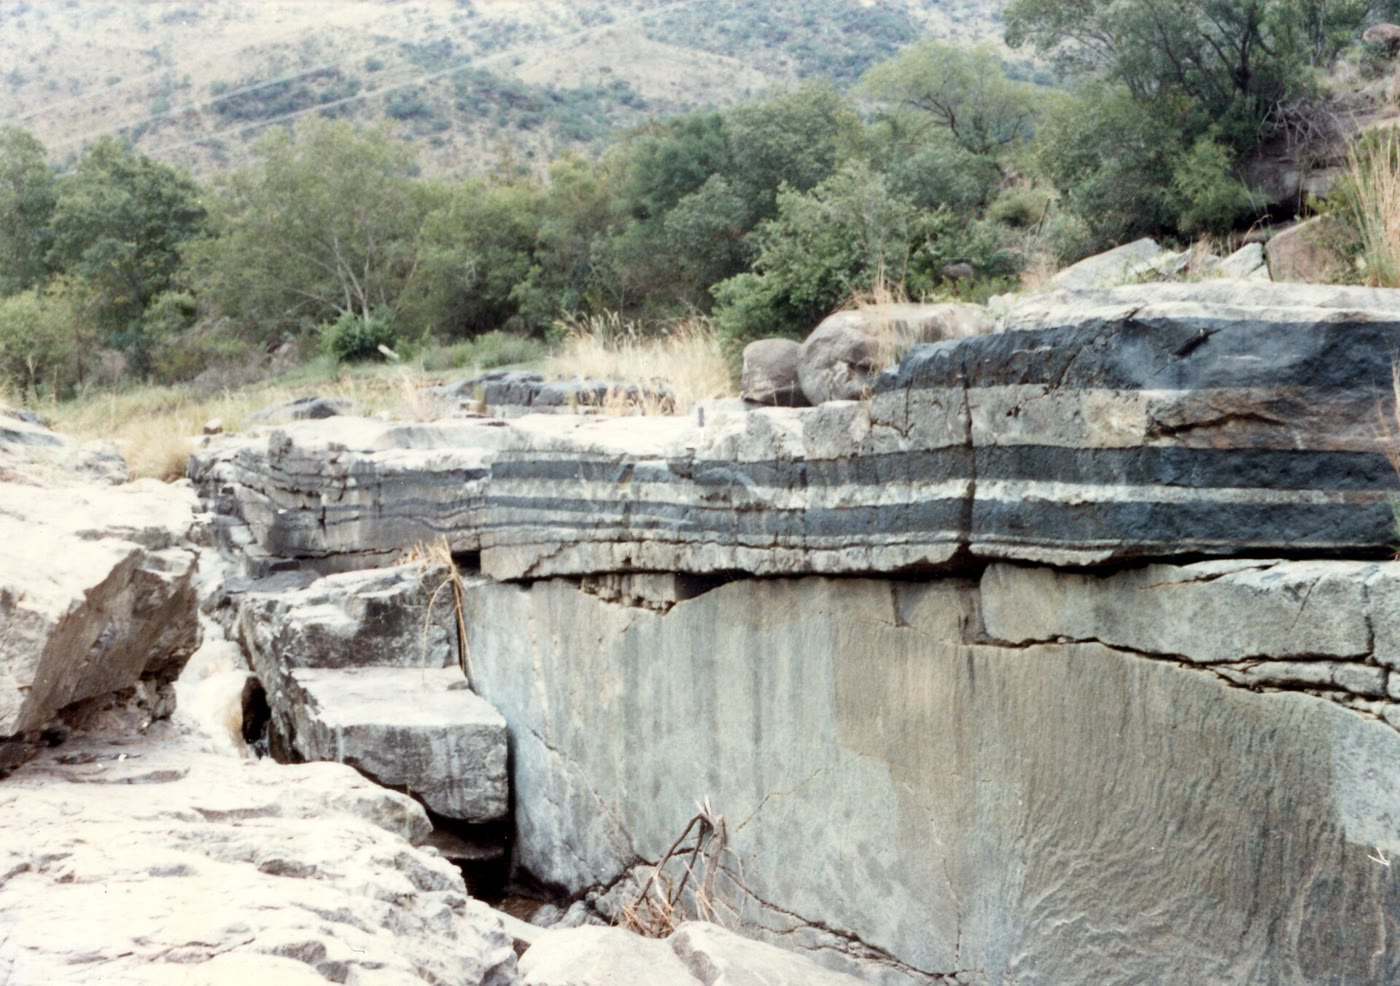
\includegraphics[height=5.2cm]{images/book4/b2-bushveld-chromitite.jpg}
\end{minipage}\hfill
\begin{minipage}[t]{0.42\linewidth}\vspace{0pt}\centering
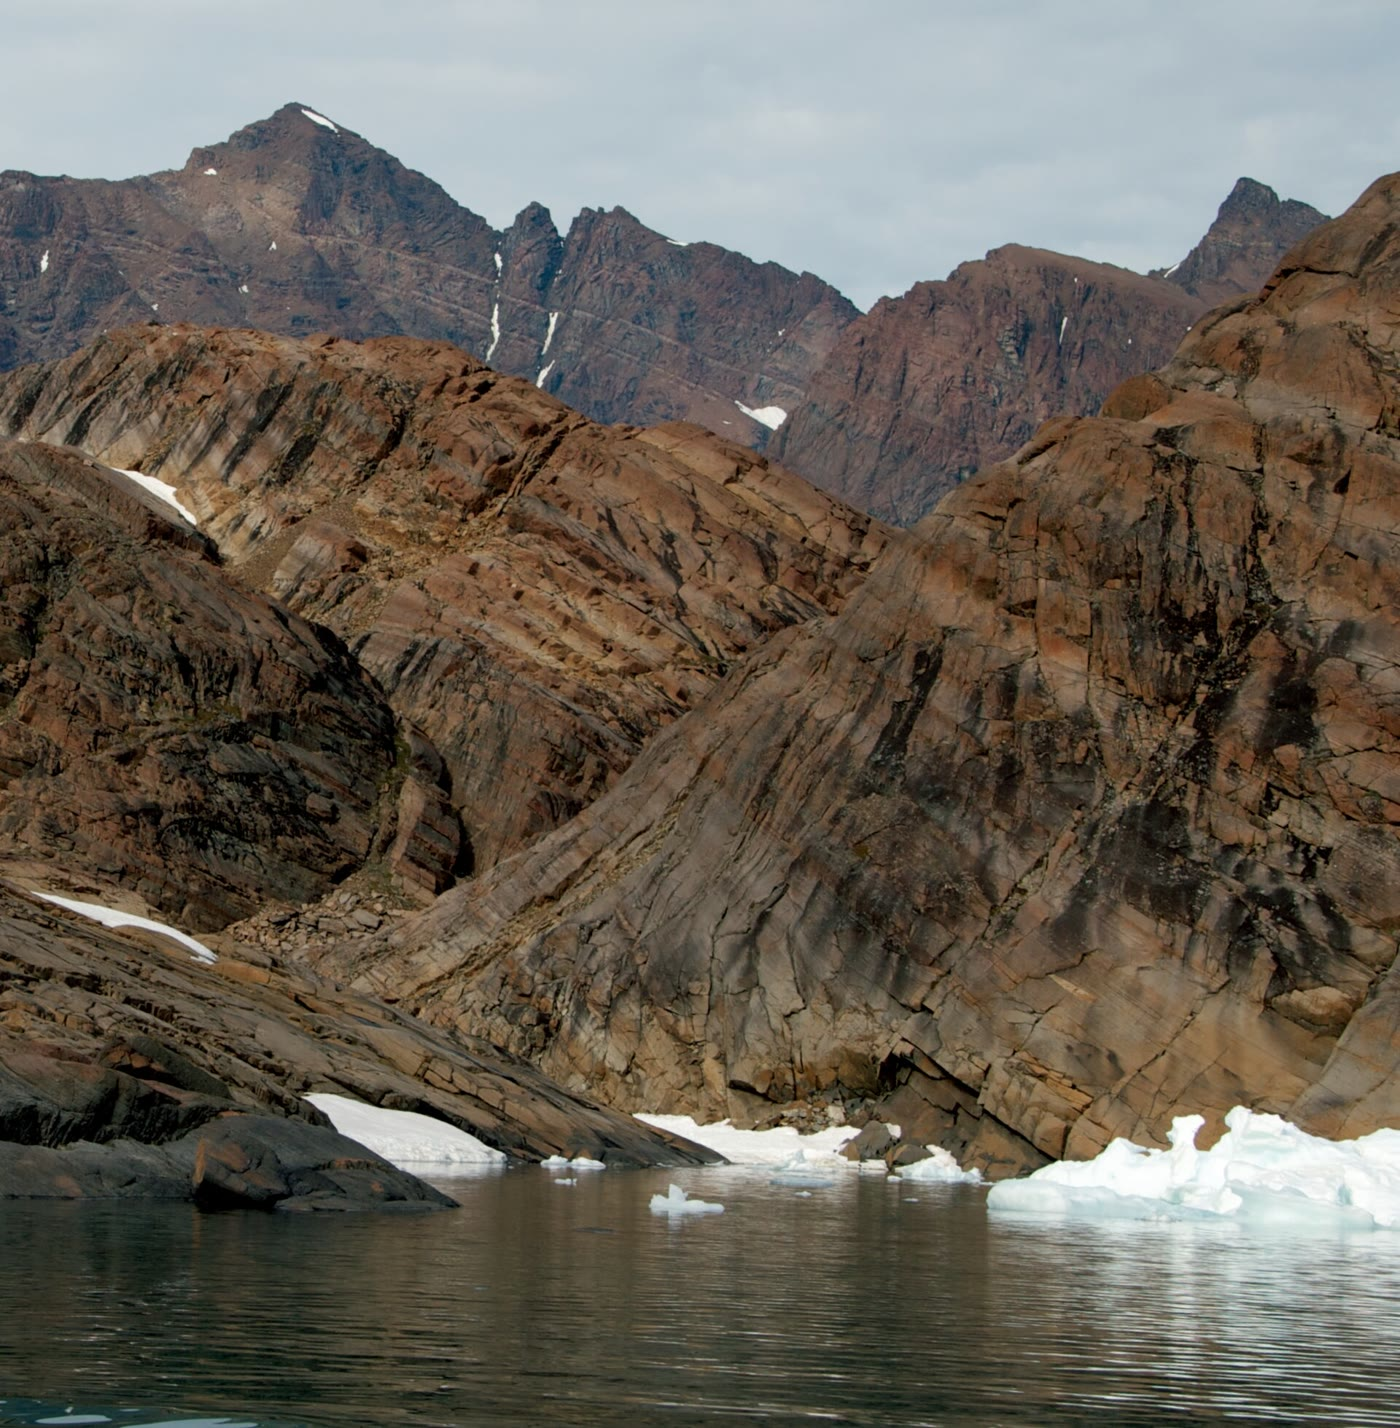
\includegraphics[height=5.2cm]{images/book4/b2-skaergaard-layering.jpg}
\end{minipage}
\par\smallskip{\small बाएँ: दक्षिण अफ़्रीका के बुशवेल्ड संकुल के क्रांतिक क्षेत्र की काली क्रोमाइटाइट और धूसर
ऐनॉर्थोसाइट परतें (फ़ोटो: Kevin Walsh, CC BY 2.0)।
दाएँ: पूर्वी ग्रीनलैंड के स्केरगार्ड अंतर्वेधन के मध्य क्षेत्र के स्तरित गैब्रो, जो
ऊपर बाएँ से नीचे दाएँ की ओर झुके हैं (फ़ोटो: C. Tegner, CC BY 4.0)।}
\end{omfigure}

\section{खुले तंत्र}\label{sec:b2:magmatic-differentiation:open}

\omterm{def:b2:magma-emplacement:magma}{मैग्मा} कक्ष शायद ही कभी बंद होता है। नीचे से नया \omterm{def:b2:magma-emplacement:magma}{मैग्मा} आता है, और कक्ष की
दीवारें ऐसी चट्टानें हैं जिन्हें \omterm{def:b2:magma-emplacement:magma}{मैग्मा} गरम कर सकता है, पिघला सकता है और घोल सकता है।

\begin{definition}[मैग्मा मिश्रण; भूपर्पटीय आत्मसातन; AFC]
\label{def:b2:magmatic-differentiation:open}
\emph{मैग्मा मिश्रण}\index{मैग्मा मिश्रण} भिन्न संघटनों वाले
दो मैग्माओं का मिलकर एक हो जाना है।
\emph{भूपर्पटीय आत्मसातन}\index{भूपर्पटीय आत्मसातन} भूपर्पटी की चट्टान का किसी \omterm{def:b2:magma-emplacement:magma}{मैग्मा} में समावेश है,
दीवार की चट्टान या उसमें गिरे खंडों के पिघलने और विलयन द्वारा।
\emph{आत्मसातन--भिन्नात्मक क्रिस्टलन}\index{आत्मसातन--भिन्नात्मक क्रिस्टलन} (AFC)
एक ही कक्ष में इन दोनों का संयोजन है: \omterm{def:b2:magma-emplacement:magma}{मैग्मा} क्रिस्टलित होता है, और मुक्त हुई
गुप्त ऊष्मा दीवार की चट्टान को पिघलाती और आत्मसात करती है।
\end{definition}

\begin{proposition}[मिश्रण सांद्रताओं में रैखिक है]\label{prop:b2:magmatic-differentiation:mixing}
\omterm{def:b2:magma-emplacement:magma}{मैग्मा} A के द्रव्यमान-अंश $s$ और \omterm{def:b2:magma-emplacement:magma}{मैग्मा} B के $1-s$ के मिश्रण की हर
सांद्रता $C = sC_A + (1-s)C_B$ होती है: एक सांद्रता के विरुद्ध दूसरी के किसी भी आरेख पर
मिश्रण A से B तक के सीधे खंड पर स्थित होते हैं, और उत्तोलक नियम
$s$ देता है।
\end{proposition}

\begin{proof}
हर तत्त्व संरक्षित रहता है: $C(m_A + m_B) = m_AC_A + m_BC_B$; $m_A + m_B$ से भाग दीजिए।
\end{proof}

मिश्रण और क्रिस्टल-निष्कासन दोनों हार्कर आरेखों पर सीधी रेखाएँ खींचते हैं; समस्थानिक
अनुपात उन्हें अलग करते हैं। क्रिस्टलन समस्थानिक अनुपात नहीं बदलता, जबकि
भिन्न अनुपात वाली चट्टान के साथ मिश्रण उसे बदलता है, \cref{ch:b2:isotope-geochemistry}
के अतिपरवलय के अनुदिश। इसलिए किसी ज्वालामुखीय अनुक्रम में सिलिका के साथ $^{87}$Sr/$^{86}$Sr की वृद्धि
आत्मसातन का चिह्न है।

\begin{proposition}[भिन्नात्मक क्रिस्टलन के साथ आत्मसातन]
\label{prop:b2:magmatic-differentiation:afc}
एक \omterm{def:b2:magma-emplacement:magma}{मैग्मा} किसी तत्त्व के लिए समग्र विभाजन गुणांक $D$ वाले क्रिस्टल क्रिस्टलित करता है
और सांद्रता $C_a$ वाली दीवार-चट्टान को क्रिस्टलन की दर के $r$ गुना दर से
आत्मसात करता है ($r \ne 1$)। $F$ को \omterm{def:b2:magma-emplacement:magma}{मैग्मा} का उसके प्रारंभिक द्रव्यमान के सापेक्ष द्रव्यमान
और $z = (r + D - 1)/(r - 1)$ लेकर,
\[
\frac{C}{C_0} = F^{-z} + \frac{r}{r - 1 + D}\,\frac{C_a}{C_0}\,\bigl(1 - F^{-z}\bigr).
\]
$r = 0$ के लिए यह रैले नियम है। \omterm{def:b2:magma-emplacement:magma}{मैग्मा} में तत्त्व का समस्थानिक अनुपात
प्रारंभिक \omterm{def:b2:magma-emplacement:magma}{मैग्मा} और दीवार-चट्टान के अनुपातों का माध्य है, जिसे
इस योग के दो पदों से भारित किया गया है।
\end{proposition}

\begin{proof}
प्रति इकाई प्रारंभिक द्रव्यमान, जब द्रव्यमान $\mathrm dm_c$ क्रिस्टलित होता है, तो द्रव्यमान
$r\,\mathrm dm_c$ आत्मसात होता है और \omterm{def:b2:magma-emplacement:magma}{मैग्मा} का द्रव्यमान $\mathrm dM =
-(1-r)\,\mathrm dm_c$ से बदलता है। तत्त्व का संतुलन $\mathrm d(MC) = rC_a\,\mathrm dm_c -
DC\,\mathrm dm_c$ है। बाएँ पक्ष का प्रसार करके और $\mathrm dm_c$ के स्थान पर
$-\mathrm dM/(1-r)$ रखकर,
\[
M\frac{\mathrm dC}{\mathrm dM} = -C - \frac{rC_a - DC}{1-r}
= \frac{(r - 1 + D)\,C - rC_a}{1 - r} = -z\,\bigl(C - C^*\bigr),
\qquad C^* = \frac{rC_a}{r - 1 + D}.
\]
अतः $\mathrm d(C - C^*)/(C - C^*) = -z\,\mathrm dM/M$, और $C - C^*$
$M^{-z}$ के समानुपाती है; चूँकि $C = C_0$ है जब $M = 1$, अतः $C = C^* + (C_0 - C^*)F^{-z}$, जो
सूत्र ही है। $r = 0$ के लिए $z = 1 - D$ और $C^* = 0$। जो परमाणु
प्रारंभिक \omterm{def:b2:magma-emplacement:magma}{मैग्मा} से आते हैं वे $C_a = 0$ के साथ उसी समीकरण का पालन करते हैं, अतः उनकी सांद्रता
$C_0F^{-z}$ है; शेष दीवार से आते हैं: इसी से समस्थानिक अनुपातों का भारण।
\end{proof}

डीपाओलो ने ये समीकरण 1981 में दिए, और वे भूपर्पटी से गुज़रते हुए संदूषित हुए \omterm{def:b2:magma-emplacement:magma}{मैग्मा} का
मानक मॉडल हैं। उनमें एक ऊष्मीय बाध्यता छिपी है। चट्टान को आत्मसात करने की
ऊष्मा क्रिस्टलों की गुप्त ऊष्मा से आती है: भूपर्पटी को
150 से \qty{1150}{\celsius} तक गरम करने में लगभग \qty{1}{kJ/g} लगते हैं, उसे पिघलाने में \qty{300}{J/g},
जबकि क्रिस्टलित होता \omterm{def:b2:magma-emplacement:magma}{मैग्मा} लगभग \qty{400}{J/g} देता है; अतः आत्मसात हुई चट्टान के हर ग्राम के लिए
लगभग \qty{3.25}{g} \omterm{def:b2:magma-emplacement:magma}{मैग्मा} को क्रिस्टलित होना पड़ता है, और $r$ 1 से काफ़ी कम है।
विलकॉक्स ने पारीकुटिन के लिए यही परिकलन किया: उनके \qty{25.4}{g} क्वार्ट्ज़
मॉन्ज़ोनाइट को, जो लगभग \qty{200}{\celsius} पर लिया गया, लगभग \qty{31350}{J} चाहिए थे, ताकि वह
\qty{1100}{\celsius} तक गरम होकर पिघल सके; यह लगभग
\qty{85}{g} प्लैजियोक्लेज़ के क्रिस्टलन की ऊष्मा है, जो उनके द्रव्यमान-संतुलन द्वारा हटाए गए \qty{12.5}{g} क्रिस्टलों से कहीं अधिक है।
फूटा हुआ \omterm{def:b2:magma-emplacement:magma}{मैग्मा} अपने आत्मसातन की कीमत स्वयं नहीं चुका सकता था:
ऊष्मा फूटे हुए \omterm{def:b2:magma-emplacement:magma}{मैग्मा} से बड़े किसी मैग्मा-पिंड से आई होगी,
जो दृष्टि से ओझल क्रिस्टलित हो रहा था (\cref{exo:b2:magmatic-differentiation:11})।
% ledger: depaolo81:afc, white09:afc-heat, wilcox54:heat, wilcox54:mass-balance

\begin{omfigure}
\centering
\begin{tikzpicture}
\begin{axis}[omrecord, name=left, width=0.47\linewidth, height=5.4cm,
  xmin=0.3, xmax=1, ymin=0.3, ymax=1.05, x dir=reverse,
  xlabel={शेष मैग्मा $F$}, ylabel={Sr: $C/C_0$},
  tick label style={font=\scriptsize}, label style={font=\small}]
\addplot[thick, black] table[x=F, y=srC_r0] {figdata/out/bachelor-2-differentiation-afc.dat};
\addplot[thick, blue!70!black] table[x=F, y=srC_r02] {figdata/out/bachelor-2-differentiation-afc.dat};
\addplot[thick, red!70!black] table[x=F, y=srC_r05] {figdata/out/bachelor-2-differentiation-afc.dat};
\end{axis}
\begin{axis}[omrecord, at={(left.east)}, anchor=west, xshift=1.7cm,
  width=0.47\linewidth, height=5.4cm,
  xmin=0.3, xmax=1, ymin=0.703, ymax=0.716, x dir=reverse,
  xlabel={शेष मैग्मा $F$}, ylabel={$^{87}$Sr/$^{86}$Sr},
  y tick label style={/pgf/number format/fixed, /pgf/number format/precision=3},
  legend style={font=\scriptsize, at={(0.03,0.97)}, anchor=north west},
  tick label style={font=\scriptsize}, label style={font=\small}]
\addplot[thick, black] table[x=F, y=iso_r0] {figdata/out/bachelor-2-differentiation-afc.dat};
\addlegendentry{$r = 0$}
\addplot[thick, blue!70!black] table[x=F, y=iso_r02] {figdata/out/bachelor-2-differentiation-afc.dat};
\addlegendentry{$r = 0.2$}
\addplot[thick, red!70!black] table[x=F, y=iso_r05] {figdata/out/bachelor-2-differentiation-afc.dat};
\addlegendentry{$r = 0.5$}
\end{axis}
\end{tikzpicture}
\par\smallskip{\small स्ट्रॉन्शियम के लिए \omterm{def:b2:magmatic-differentiation:crystallisation}{भिन्नात्मक क्रिस्टलन} के साथ आत्मसातन
($D = 1.5$, \omterm{def:b2:magma-emplacement:magma}{मैग्मा} की आधी स्ट्रॉन्शियम वाली दीवार-चट्टान, जिसका
$^{87}$Sr/$^{86}$Sr = 0.7200 है, \omterm{def:b2:magma-emplacement:magma}{मैग्मा} 0.7035; दृष्टांत-मान)। बाएँ:
आत्मसातन-दर $r$ बढ़ने के साथ सांद्रता अधिक तेज़ी से गिरती है, क्योंकि दीवार-चट्टान
कम स्ट्रॉन्शियम लाती है और उसी $F$ के लिए अधिक क्रिस्टल बनते हैं। दाएँ: समस्थानिक
अनुपात, जो अकेले क्रिस्टलन से नहीं बदलता ($r = 0$), दीवार के अनुपात की ओर चढ़ता है।}
\end{omfigure}

\section{मंडलित क्रिस्टलों को पढ़ना}\label{sec:b2:magmatic-differentiation:zoning}

\begin{definition}[संघटनात्मक मंडलन]\label{def:b2:magmatic-differentiation:zoning}
किसी ठोस विलयन के क्रिस्टल में \emph{संघटनात्मक मंडलन}\index{संघटनात्मक मंडलन}
होता है जब उसका संघटन क्रोड से किनारे तक बदलता है; यह मंडलन उस बदलते द्रव को दर्ज करता है
जिससे क्रमिक परतें उगीं। मंडलन \emph{सामान्य} होता है जब किनारा
निम्न-तापमान घटक (प्लैजियोक्लेज़ में सोडियम) में अधिक समृद्ध हो, \emph{उलटा} जब वह
उच्च-तापमान घटक में अधिक समृद्ध हो, और \emph{दोलनी} जब यह बारी-बारी से बदलता हो।
\end{definition}

मंडलित क्रिस्टल रंगे हाथ पकड़ा गया \omterm{def:b2:magmatic-differentiation:crystallisation}{भिन्नात्मक क्रिस्टलन} है: उसका क्रोड
बाद के द्रव के साथ फिर से साम्य में नहीं आया। नीचे का चित्र बोवेन के लूप पर
\qty{50}{\percent} एनॉर्थाइट वाले द्रव से उगते प्लैजियोक्लेज़ का परिकलन करता है।
साम्य में क्रिस्टल समांगी रहते हैं और \qty{50}{\percent} पर समाप्त होते हैं; पूर्ण
\omterm{def:b2:magmatic-differentiation:crystallisation}{भिन्नात्मक क्रिस्टलन} में हर नई परत निरंतर अधिक सोडियमी द्रव के साथ साम्य में होती है,
और अंतिम क्रिस्टलों का किनारा लगभग शुद्ध एल्बाइट होता है। कैल्शियमी क्रोड से सोडियमी किनारे तक का
सामान्य मंडलन वही है जिसकी बोवेन की श्रेणी ठंडे होते \omterm{def:b2:magma-emplacement:magma}{मैग्मा} के लिए भविष्यवाणी करती है। उलटा
मंडल, यानी सोडियमी मंडल के बाहर एक कैल्शियमी पट्टी, बताता है कि क्रिस्टल अचानक
अधिक गरम या अधिक कैल्शियमी द्रव में डूब गया: प्रायः यह नए \omterm{def:b2:magma-emplacement:magma}{मैग्मा} का आगमन, यानी कक्ष में
मिश्रण, होता है।
% ledger: bowen13:plagioclase, earle:bowen (Book 2)

\begin{omfigure}
\centering
\begin{tikzpicture}
\begin{axis}[omrecord, width=0.78\linewidth, height=6cm,
  xmin=0, xmax=1, ymin=0, ymax=90,
  xlabel={क्रिस्टलित हुए द्रव का अंश},
  ylabel={एनॉर्थाइट (\unit{\percent}, आणविक)},
  legend style={font=\scriptsize, at={(0.02,0.02)}, anchor=south west},
  tick label style={font=\scriptsize}, label style={font=\small}]
\addplot[very thick, red!70!black] table[x=x, y=an_frac] {figdata/out/bachelor-2-differentiation-zoning.dat};
\addlegendentry{भिन्नात्मक: बनती परत}
\addplot[thick, gray, densely dotted] table[x=x, y=an_liq_frac] {figdata/out/bachelor-2-differentiation-zoning.dat};
\addlegendentry{भिन्नात्मक: द्रव}
\addplot[very thick, blue!70!black, dashed] table[x=x, y=an_eq] {figdata/out/bachelor-2-differentiation-zoning.dat};
\addlegendentry{साम्य: क्रिस्टल}
\end{axis}
\end{tikzpicture}
\par\smallskip{\small \qty{50}{\percent} एनॉर्थाइट वाले द्रव से क्रिस्टलित होता प्लैजियोक्लेज़,
बोवेन (1913) के लूप पर परिकलित। \omterm{def:b2:magmatic-differentiation:crystallisation}{भिन्नात्मक क्रिस्टलन} में
क्रिस्टलों की क्रमिक परतें, क्रोड (बाएँ) से किनारे (दाएँ) तक, निरंतर अधिक
सोडियमी होती जाती हैं, और लगभग \qty{82}{\percent} क्रिस्टलित हो जाने पर द्रव एल्बाइट तक पहुँचता है;
\omterm{def:b2:magmatic-differentiation:crystallisation}{साम्य क्रिस्टलन} में क्रिस्टल एकसमान रहते हैं और उस द्रव के संघटन के साथ
समाप्त होते हैं जिससे वे बने।}
\end{omfigure}

\begin{inthelab}[मंडलित क्रिस्टलों को पढ़ना]
शैलिकीविद मंडलन को पहले आड़े ध्रुवकों के बीच पढ़ते हैं, जहाँ किसी
प्लैजियोक्लेज़ के मंडल थोड़े भिन्न कोणों पर विलोपित होते हैं और संकेंद्री पट्टियों के रूप में दिखते हैं।
फिर वे उसे मापते हैं: इलेक्ट्रॉन माइक्रोप्रोब (\cref{ch:b2:field-lab-methods-2})
क्रोड से किनारे तक एक अनुप्रस्थ पथ के अनुदिश कुछ माइक्रोमीटर चौड़े बिंदुओं का विश्लेषण करता है, और
कैल्शियम और सोडियम के मानचित्र मंडलों को सीधे दिखाते हैं। ऐसी प्रोफ़ाइल से वे
उस द्रव का संघटन परिकलित करते हैं जिससे हर मंडल उगा, ऊपर के चित्र के लूप से या
विभाजन गुणांकों से, और वे उलटे मंडलों को कक्ष के पुनर्भरणों की संख्या के रूप में
गिनते हैं। उसी अनुप्रस्थ पथ के अनुदिश लेज़र
अपक्षरण से मापे गए \omterm{def:b2:elements-in-the-earth:trace}{अनुरेखी तत्त्व}, और मंडल-दर-मंडल मापे गए समस्थानिक अनुपात,
एक ही क्रिस्टल के इतिहास में क्रिस्टलन, मिश्रण और आत्मसातन को अलग करते हैं।
\end{inthelab}

\section{अभ्यास}

\begin{exercise}[$\star$]\label{exo:b2:magmatic-differentiation:1}
प्लैजियोक्लेज़ों पर बोवेन के मापों का उपयोग कीजिए (सॉलिडस / लिक्विडस, \unit{\celsius}):
An$_{100}$ 1550 / 1550; An$_{83.3}$ 1465 / 1521; An$_{66.7}$ 1372 / 1490; An$_{50}$
1287 / 1450; An$_{33.3}$ 1205 / 1394; An$_{20}$ लिक्विडस 1334; An$_{11.1}$ लिक्विडस
1265, और पड़ोसी बिंदुओं के बीच रैखिक अंतर्वेशन कीजिए। \qty{50}{\percent}
एनॉर्थाइट वाला एक द्रव साम्य में ठंडा होता है। (क) वह किस तापमान पर
क्रिस्टलित होने लगता है, और पहले क्रिस्टल का संघटन क्या है? (ख)
\qty{1394}{\celsius} पर द्रव और क्रिस्टलों के संघटन क्या हैं,
और कितना द्रव्यमान-अंश क्रिस्टलित हो चुका है (मोल-अंशों को ऐसे लीजिए मानो वे द्रव्यमान-अंश
हों)? (ग) द्रव की अंतिम बूँद का संघटन क्या है?
\end{exercise}
% ledger: bowen13:plagioclase

\begin{exercise}[$\star$]\label{exo:b2:magmatic-differentiation:2}
एक गैब्रोई \omterm{def:b2:magmatic-differentiation:cumulate}{क्यूम्यूलेट} में \qty{50}{\percent} प्लैजियोक्लेज़, \qty{35}{\percent}
क्लाइनोपाइरॉक्सीन और \qty{15}{\percent} ओलिवीन है। विभाजन गुणांकों
(ओलिवीन / क्लाइनोपाइरॉक्सीन / प्लैजियोक्लेज़) Sr 0.000063 / 0.157 / 2.7, Zr 0.00068 /
0.195 / 0.001 और Rb 0.000044 / 0.0033 / 0.025 के साथ, हर तत्त्व का समग्र विभाजन
गुणांक परिकलित कीजिए, और बताइए कि कौन-सा संगत है।
\end{exercise}
% ledger: white07:kd-basalt

\begin{exercise}[$\star$]\label{exo:b2:magmatic-differentiation:3}
\cref{exo:b2:magmatic-differentiation:2} का \omterm{def:b2:magmatic-differentiation:cumulate}{क्यूम्यूलेट} एक बेसाल्ट से \omterm{def:b2:magmatic-differentiation:crystallisation}{भिन्नात्मक क्रिस्टलन} द्वारा तब तक क्रिस्टलित होता है,
जब तक आधा द्रव शेष न रह जाए। (क) द्रव में Sr, Zr और Rb में से हर एक किस गुणक से बदला है
(समग्र गुणांक 1.40, 0.069 और 0.014 लीजिए)? (ख) अनुपात Zr/Rb किस गुणक से
बदला है? अनुपातों वाले उपप्रमेय के आधार पर टिप्पणी कीजिए।
\end{exercise}
% ledger: white07:kd-basalt

\begin{exercise}[$\star$]\label{exo:b2:magmatic-differentiation:4}
पारीकुटिन के पहले लावा (फ़रवरी 1943) में \qty{55.04}{\percent} \ce{SiO2},
\qty{5.68}{\percent} \ce{MgO} और \qty{0.85}{\percent} \ce{K2O} था; अंतिम (फ़रवरी
1952) में 60.07, 3.73 और \qty{1.67}{\percent}। (क) हर ऑक्साइड का परिवर्तन परिकलित कीजिए।
(ख) पोटाश क्रिस्टलित होने वाले किसी भी खनिज में प्रवेश नहीं करता। यदि यह केवल
\omterm{def:b2:magmatic-differentiation:crystallisation}{भिन्नात्मक क्रिस्टलन} से सांद्रित हुआ होता, तो द्रव का कितना अंश शेष रहा होता?
(ग) विलकॉक्स का द्रव्यमान-संतुलन केवल लगभग \qty{12.5}{g} क्रिस्टल हटाता है, \omterm{def:b2:magma-emplacement:magma}{मैग्मा} के हर
\qty{100}{g} पर। यह तुलना क्या संकेत देती है?
\end{exercise}
% ledger: wilcox54:table2, wilcox54:mass-balance

\begin{exercise}[$\star\star$]\label{exo:b2:magmatic-differentiation:5}
भिन्नात्मक और \omterm{def:b2:magmatic-differentiation:crystallisation}{साम्य क्रिस्टलन} की तुलना कीजिए: दोनों नियमों से $C_L/C_0$ परिकलित कीजिए
(क) निकेल के लिए, $D = 5$, जब द्रव का \qty{20}{\percent} क्रिस्टलित हो चुका हो; (ख)
एक \omterm{def:b2:elements-in-the-earth:partition}{असंगत तत्त्व} के लिए, $D = 0.01$, जब \qty{90}{\percent} क्रिस्टलित हो चुका हो।
(ग) $F \to 0$ होने पर दोनों नियमों की सीमाएँ क्या हैं? कौन-सा नियम किसी द्रव से
\omterm{def:b2:elements-in-the-earth:partition}{संगत तत्त्व} को पूरी तरह निकाल सकता है?
\end{exercise}

\begin{exercise}[$\star\star$]\label{exo:b2:magmatic-differentiation:6}
(क) \ce{MgO}, \ce{FeO} और \ce{SiO2} के द्रव्यमान-प्रतिशत परिकलित कीजिए, ओलिवीन
Fo$_{80}$, $(\ce{Mg}_{0.8}\ce{Fe}_{0.2})_2\ce{SiO4}$ में ($M$ = 40.30, 71.84 और
\qty{60.08}{g/mol})। (ख) \qty{10.0}{\percent} \ce{MgO} और
\qty{49.0}{\percent} \ce{SiO2} वाला एक बेसाल्ट केवल यही ओलिवीन तब तक क्रिस्टलित करता है जब तक उसके द्रव में
\qty{8.0}{\percent} \ce{MgO} न रह जाए। ओलिवीन का कितना द्रव्यमान-अंश हटाया गया? (ग) तब
द्रव में सिलिका की मात्रा क्या है?
\end{exercise}

\begin{exercise}[$\star\star$]\label{exo:b2:magmatic-differentiation:7}
स्केरगार्ड अंतर्वेधन के लिए $F = \num{1.091e-7}H^2 - \num{5.9064e-4}H + 0.7678$।
(क) $F$ परिकलित कीजिए, $H = 0$, 1000 और \qty{2000}{m} पर। (ख) किस ऊँचाई पर $F = 0$ है?
(ग) अनावृत तल-अनुक्रम का आधार बनने से पहले \omterm{def:b2:magma-emplacement:magma}{मैग्मा} का कितना अंश क्रिस्टलित हो चुका था,
और वह कहाँ हो सकता है?
\end{exercise}
% ledger: tegner23:skaergaard

\begin{exercise}[$\star\star$]\label{exo:b2:magmatic-differentiation:8}
स्केरगार्ड परिच्छेद के अनुदिश माध्यिका \omterm{def:b2:magmatic-differentiation:cumulate}{क्यूम्यूलेट} में \qty{177}{ppm} Ni होता है
$F = 0.70$ पर (निचला क्षेत्र a), \qty{54}{ppm} $F = 0.29$ पर (मध्य क्षेत्र) और
\qty{6.2}{ppm} $F = 0.17$ पर (ऊपरी क्षेत्र a)। (क) यह मानकर कि \omterm{def:b2:magmatic-differentiation:cumulate}{क्यूम्यूलेटों} में
उनके द्रव के निकेल का $D$ गुना होता है और द्रव रैले नियम का पालन करता है,
पहले दो स्तरों के बीच आभासी $D$ परिकलित कीजिए। (ख) अंतिम दो के बीच भी यही कीजिए।
(ग) आभासी $D$ के बदलने का कारण क्या हो सकता है?
\end{exercise}
% ledger: data:b4-skaergaard

\begin{exercise}[$\star\star$]\label{exo:b2:magmatic-differentiation:9}
विलकॉक्स के उत्तर की जाँच कीजिए: पहले लावा के आधारद्रव्य के \qty{100}{g} (\ce{SiO2}
55.53, \ce{MgO} 4.66, \ce{K2O} \qty{0.88}{\percent}) में \qty{25.4}{g} औसत
ज़ेनोलिथ (72.48, 0.77, 3.64) जोड़िए, \qty{2.9}{g} ओलिवीन Fo$_{80}$ (39.19, 42.06, 0) घटाइए
और \qty{9.6}{g} प्लैजियोक्लेज़ An$_{70}$ (50.54, 0, 0) घटाइए। (क) कितना द्रव्यमान शेष रहता है?
(ख) उसके \ce{SiO2}, \ce{MgO} और \ce{K2O} परिकलित कीजिए और उनकी तुलना लावा 19 के
आधारद्रव्य (60.16, 3.19 और \qty{1.75}{\percent}) से कीजिए। (ग) कौन-सा ऑक्साइड सबसे कम मेल खाता है?
\end{exercise}
% ledger: wilcox54:groundmass, wilcox54:xenoliths, wilcox54:mass-balance

\begin{exercise}[$\star\star\star$]\label{exo:b2:magmatic-differentiation:10}
एक \omterm{def:b2:magma-emplacement:magma}{मैग्मा} क्रिस्टलित होते हुए $r = 0.2$ पर दीवार-चट्टान को आत्मसात करता है, जहाँ $D_{\ce{Sr}} =
1.5$, $C_a/C_0 = 0.5$, प्रारंभिक $^{87}$Sr/$^{86}$Sr = 0.7035 और दीवार-चट्टान का 0.7200 है।
(क) $z$, $F^{-z}$ और $C/C_0$ परिकलित कीजिए, $F = 0.7$ पर। (ख) उसी $F$ पर शुद्ध \omterm{def:b2:magmatic-differentiation:crystallisation}{भिन्नात्मक
क्रिस्टलन} से तुलना कीजिए, और अंतर को हर स्थिति में बने क्रिस्टलों के द्रव्यमान से समझाइए।
(ग) \omterm{def:b2:magma-emplacement:magma}{मैग्मा} का $^{87}$Sr/$^{86}$Sr परिकलित कीजिए।
\end{exercise}

\begin{exercise}[$\star\star\star$]\label{exo:b2:magmatic-differentiation:11}
पारीकुटिन के लिए विलकॉक्स के ऊष्मा-बजट का अनुसरण कीजिए। (क) एक ग्राम क्वार्ट्ज़
मॉन्ज़ोनाइट को 200 से \qty{1100}{\celsius} तक जाने के लिए (ऊष्मा धारिता
\qty{1.1}{J/(g.K)}) और फिर पिघलने के लिए (\qty{250}{J/g}) कितनी ऊष्मा चाहिए? (ख)
\qty{25.4}{g} के लिए कितनी? (ग) प्लैजियोक्लेज़ An$_{70}$ (गुप्त ऊष्मा \qty{370}{J/g}) का कितना
द्रव्यमान इसकी आपूर्ति के लिए क्रिस्टलित होना चाहिए? (घ) द्रव्यमान-संतुलन के \qty{12.5}{g} क्रिस्टलों से
तुलना कीजिए, आत्मसातन और क्रिस्टलन का अनुपात $r$ परिकलित कीजिए, और बताइए कि
इसका क्या निहितार्थ है।
\end{exercise}
% ledger: wilcox54:heat, white09:afc-heat

\begin{exercise}[$\star\star\star$]\label{exo:b2:magmatic-differentiation:12}
\qty{250}{ppm} Ni वाला एक बेसाल्ट पहले केवल ओलिवीन ($D = 5$) क्रिस्टलित करता है, जब तक
$F = 0.8$ न हो जाए, फिर प्लैजियोक्लेज़ और क्लाइनोपाइरॉक्सीन के साथ ओलिवीन (समग्र $D = 1.5$)। (क)
हर चरण में निकेल जिस गुणक से बदलता है वह परिकलित कीजिए, और $F = 0.5$ पर
द्रव में निकेल की मात्रा भी। (ख) $D = 5$ वाले एक अकेले नियम ने क्या भविष्यवाणी की होती?
(ग) समझाइए कि रैले नियम चरणों में क्यों लागू करना पड़ता है।
\end{exercise}

\section{समस्या: वह अंतर्वेधन जिसने अपना इतिहास स्वयं लिखा}

\begin{problem}[{सप्ताहांत समस्या --- गैब्रो की परतों से उसके मैग्मा के उस अंश तक जो
अंत में भी द्रव था}]
\label{pb:b2:magmatic-differentiation:1}
एक (काल्पनिक) स्तरित गैब्रो \omterm{def:b2:magma-emplacement:bodies}{सिल} एक बेसाल्ट से क्रिस्टलित हुई, जिसका \omterm{def:b2:magma-emplacement:aureole}{शीतित किनारा}
जनक संघटन देता है: \ce{SiO2} 49.5, \ce{Al2O3} 16.0, \ce{FeO} 10.0,
\ce{MgO} 9.0, \ce{CaO} 11.5, \ce{Na2O} 2.5, \ce{K2O} \qty{0.30}{\percent};
\qty{150}{ppm} Ni और \qty{80}{ppm} Zr। निचले क्षेत्र के \omterm{def:b2:magmatic-differentiation:cumulate}{क्यूम्यूलेट}
\qty{20}{\percent} ओलिवीन, \qty{50}{\percent} प्लैजियोक्लेज़ और \qty{30}{\percent}
क्लाइनोपाइरॉक्सीन से बने हैं; उस स्तर के ऊपर जहाँ ओलिवीन लुप्त होता है,
\qty{55}{\percent} प्लैजियोक्लेज़ और \qty{45}{\percent} क्लाइनोपाइरॉक्सीन से। विभाजन गुणांक लीजिए
(ओलिवीन / प्लैजियोक्लेज़ / क्लाइनोपाइरॉक्सीन) Ni 5.0 / 0 / 2.0 और Zr 0.0007 / 0.001 /
0.195। खनिज संघटन (\unit{\percent}): ओलिवीन \ce{MgO} 42.06, \ce{CaO} 0,
\ce{Al2O3} 0, \ce{SiO2} 39.19; प्लैजियोक्लेज़ 0, 14.36, 31.70, 50.54; क्लाइनोपाइरॉक्सीन
16.0, 20.5, 3.0, 51.5। सूक्ष्म-कणिक चट्टान के एक \omterm{def:b2:magma-emplacement:bodies}{डाइक} में, जिसे सबसे ऊपरी परत के
क्रिस्टलित होते समय कक्ष से पोषण मिला,
\ce{SiO2} 50.0, \ce{Al2O3} 14.1, \ce{FeO} 16.7, \ce{MgO} 4.9, \ce{CaO} 7.3,
\ce{Na2O} 3.4, \ce{K2O} \qty{0.75}{\percent} और \qty{188}{ppm} Zr है।

\noindent\textbf{भाग I --- परतों के विभाजन गुणांक।}
\begin{enumerate}
\item निचले क्षेत्र में निकेल का समग्र विभाजन गुणांक परिकलित कीजिए।
\item निचले क्षेत्र में ज़िरकोनियम का गुणांक परिकलित कीजिए।
\item ऊपरी क्षेत्र में दोनों परिकलित कीजिए।
\item हर क्षेत्र में कौन-सा तत्त्व संगत है? जब ओलिवीन लुप्त हो जाता है तब क्या निकेल
संगत बना रहता है?
\item \omterm{def:b2:magmatic-differentiation:cumulate}{क्यूम्यूलेटों} का अधिकांश ज़िरकोनियम कौन-सा खनिज धारण करता है, और क्यों?
\item निचले क्षेत्र में $F$ के हर बार आधा होने पर द्रव में Ni/Zr किस गुणक से
बदलता है?
\end{enumerate}

\noindent\textbf{भाग II --- परिच्छेद में ऊपर की ओर रैले वक्र।}
\begin{enumerate}[resume]
\item सबसे निचले \omterm{def:b2:magmatic-differentiation:cumulate}{क्यूम्यूलेट} में, जो $F = 1$ पर क्रिस्टलित हुआ, आप निकेल की कितनी मात्रा की
अपेक्षा करते हैं?
\item निचले क्षेत्र का एक ऊपरी \omterm{def:b2:magmatic-differentiation:cumulate}{क्यूम्यूलेट} \qty{190}{ppm} Ni धारण करता है। वह किस $F$ पर
बना?
\item तब द्रव में ज़िरकोनियम की मात्रा क्या थी?
\item उसी $F$ पर, भिन्नात्मक और साम्य नियमों द्वारा दिए गए द्रव के निकेल की
तुलना कीजिए।
\item ओलिवीन $F = 0.55$ पर लुप्त होता है। वहाँ द्रव में निकेल की मात्रा
परिकलित कीजिए।
\item उस स्तर के ठीक नीचे और ठीक ऊपर बने \omterm{def:b2:magmatic-differentiation:cumulate}{क्यूम्यूलेटों} का निकेल परिकलित कीजिए। भूविज्ञानी
प्रोफ़ाइल में कौन-सा लक्षण देखेगा?
\item $F = 0.40$ पर द्रव और \omterm{def:b2:magmatic-differentiation:cumulate}{क्यूम्यूलेट} का निकेल परिकलित कीजिए। इस
प्रवृत्ति को समझाइए।
\end{enumerate}

\noindent\textbf{भाग III --- अंतिम द्रव का द्रव्यमान-संतुलन।}
\begin{enumerate}[resume]
\item विधि का संरक्षण समीकरण एक ऑक्साइड के लिए लिखिए, जिसमें द्रव्यमान
$x_{\mathrm{ol}}, x_{\mathrm{pl}}, x_{\mathrm{cpx}}$ जनक के हर \qty{100}{g} पर
हटाए गए हों और \omterm{def:b2:magma-emplacement:bodies}{डाइक} संतति हो।
\item इसे \ce{MgO}, \ce{CaO} और \ce{Al2O3} के लिए लिखिए।
\item $3 \times 3$ निकाय हल कीजिए।
\item जनक का कितना अंश द्रव के रूप में शेष है?
\item उत्तर की जाँच \ce{SiO2} से कीजिए: पाए गए द्रव्यमानों से द्रव की सिलिका का
पुनः परिकलन कीजिए।
\item हटाए गए खनिजों के अनुपातों की तुलना दोनों क्षेत्रों के
खनिज-संघटनों से कीजिए।
\item पोटाश किसी भी खनिज में प्रवेश नहीं करता: वह द्रव का कितना अंश देता है?
\end{enumerate}

\noindent\textbf{भाग IV --- शीर्ष पर द्रव का अंश।}
\begin{enumerate}[resume]
\item जब ओलिवीन $F = 0.55$ पर लुप्त हुआ, तब तक द्रव में ज़िरकोनियम किस गुणक से
बढ़ चुका था? तब ज़िरकोनियम की मात्रा बताइए।
\item \omterm{def:b2:magma-emplacement:bodies}{डाइक} के ज़िरकोनियम से उसके बनने के समय शेष द्रव का अंश परिकलित कीजिए,
$F = 0.55$ से ऊपरी क्षेत्र का नियम लागू करते हुए।
\item आरंभ से एक अकेले $D = 0.07$ के साथ परिकलन दोबारा कीजिए। क्या उत्तर
$D$ के विवरणों के प्रति संवेदनशील है?
\item द्रव में लोहा 10.0 से \qty{16.7}{\percent} तक बढ़ा, जबकि सिलिका मुश्किल से
बदली। कौन-से खनिज इसके लिए उत्तरदायी हैं, और यह किस प्रकार की मैग्मीय श्रेणी का
पूर्वाभास देता है (\cref{ch:b2:magmatic-series})?
\item सबसे ऊपरी \omterm{def:b2:magmatic-differentiation:cumulate}{क्यूम्यूलेट} \qty{47}{ppm} Zr धारण करते हैं। अकेले क्यूम्यूलस क्रिस्टल
द्रव के ज़िरकोनियम का $\bar D$ गुना धारण करते; फँसे द्रव का (\omterm{def:b2:magma-emplacement:bodies}{डाइक} के संघटन वाला) कितना
द्रव्यमान-अंश इस विश्लेषण की व्याख्या करता है?
\item सबसे ऊपरी परत के क्रिस्टलित होते समय मूल \omterm{def:b2:magma-emplacement:magma}{मैग्मा} का जो अंश अब भी द्रव था, उसे बताइए
(यह इस समस्या की मुख्य संख्या है), और तीनों अनुमानों की तुलना कीजिए
(मुख्य तत्त्व, पोटाश, ज़िरकोनियम)।
\end{enumerate}
\end{problem}
% ledger: white07:kd-basalt, matzen12:dni
